\section{Evaluation and Results} \label{sec:results}

%
%\paragraph{AC3 Subvolume.} For development and parameter exploration, we use the publicly-available dataset of mouse cortex known in the community as AC3. The dataset size is $1024\times1024\times75$ voxels and the resolution is $6\times6\times30~\text{nm}^3\text{/voxel}$. AC3 was acquired using serial section transmission electron microscopy (ssTEM).
%
%\paragraph{L. Cylinder.} We use the left part of the 3-cylinder mouse cortex volume of Kasthuri et al.~\cite{kasthuri2015saturated} ($2048\times2048\times50$ voxels). The tissue is dense mammalian neuropil from layers 4 and 5 of the S1 primary somatosensory cortex, acquired using serial section electron microscopy (ssEM). The dataset resolution is $3\times3\times30~\text{nm}^3\text{/voxel}$. Image data and a manually-labeled expert `ground truth' segmentation is publicly available\footnote{\scriptsize{\url{https://software.rc.fas.harvard.edu/lichtman/vast/}}}.
%
%\paragraph{CREMI.} As part of the MICCAI 2016 challenge on circuit reconstruction from electron microscopy images (CREMI), six ssTEM datasets were made publicly available\footnote{\scriptsize{\url{http://www.cremi.org}}},  each $1250\times1250\times125$ voxels. The volumes are part of an adult fruit fly (Drosophila melanogaster) brain. The resolution of all three datasets is $4\times4\times40~\text{nm}^3\text{/voxel}$. We include the CREMI A dataset for our evaluation.
%\\~\\
%We use a state-of-the-art method to create a dense automatic segmentation of the datasets.
%Membrane probabilities are generated using a convolutional neural network based on the U-net architecture~\cite{RonnebergerFB15}.
%The probabilities are used to seed watershed and generate an oversegmentation using superpixels.
%Agglomeration is then performed by the GALA active learning classifier~\cite{nunez2014graph}.
%The output of the agglomeration is shown in Fig.~\ref{fig:data}.
%
%\paragraph{MRI.} We include a label map of a T1-weighted brain MRI scan to evaluate compression on non-connectomics data. The dataset dimensions are $250\times250\times250$ voxels with a resolution of $1\times1\times1~\text{mm}^3\text{/voxel}$. This dataset is isotropic. The segmentation was obtained using the publicly available tool FreeSurfer\footnote{\scriptsize{FreeSurfer is available at \url{https://surfer.nmr.mgh.harvard.edu/}.}}.

%\subsection{Parameter Estimation}
%\paragraph{Varying Window Size.}
%\begin{figure}
%	\begin{center}
%		\includegraphics[width=0.7\textwidth]{./gfx/bockwurst_window_size.png}
%		\caption{The above plots show the effect of window size on the compression ratio. The left subplot shows the variation with window sizes $(n, n, 1)$ for $n$ ranging between $1$ and $720$. The right subplot shows the results where $z$ is no longer constrained to equal 1.}
%		\label{fig:bockwurst-window-size}
%	\end{center}
%\end{figure}
%Figure \ref{fig:bockwurst-window-size} shows the compression results of \appName on several connectomics datasets. There is a trade-off between the number of windows and the number of unique window values when varying the window size. The compression ratio generally peaks around the same window sizes across several different data sets.

We consider the following compression schemes: Compresso, Neuroglancer, Brotli, BZip2, Zlib, LZ78, LZF, LZMA, LZO, LZW, Zopfli, Zstandard, PNG, JPEG2000, and X.264. 
In addition to these stand-alone compression schemes we consider all pairs with a first stage encoding using either Compresso or Neuroglancer and a second stage using one of the general-purpose algorithms. 
Both \appName and Neuroglancer leave some redundancies that a general-purpose compressor can easily reduce; such multi-stage schemes are common in image compression. 
Table~\ref{tab:datasets} presents six connectomics, three MRI, and two image segmentation datasets used for evaluation. 
Compresso works for any arbitrary 2-D and 3-D window dimensions. We achieve the results in this section using an 8x8x1 window.

%We consider the following compression schemes: \appName, Neuroglancer, Run-Length Encoding (RLE), Brotli, BZip2, Zlib, LZ78, LZF, LZMA, LZO, LZW, Zopfli, Zstandard, PNG, JPEG2000, and X.264. In addition to these stand-alone compression schemes we consider all pairs between \appName, Neuroglancer, RLE, and the following general-purpose algorithms: Brotli, BZip2, ZLIB, LZ78, LZF, LZMA, LZO, LZW, Zopfli, Zstandard.

The combination of \appName and LZMA provides superior compression on all connectomics datasets (Tab.~\ref{tab:datasets}). Figure~\ref{fig:compression_ratios} shows the compression ratios for every compressor on segmentation data. For example, \appName achieves a compression ratio of over 950x on $L. Cylinder$ reducing the 10 gigabyte volume to 10.5 megabytes. LZMA performs very well by itself and paired with any encoding strategy. X.264 performs surprisingly poorly on these datasets, in part because

\begin{table}[!th]
\begin{minipage}{\textwidth}
\small
\caption{For evaluation, we use the following publicly available datasets. Segmentations were obtained using a combination of U-net~\cite{ronneberger2015u} and watershed, semi-automatic, or manually. Compresso paired with LZMA yields the best compression ratio on all datasets indicated by an asterisk (\textbf{*}). Neuroglancer paired with LZMA achieved the best compression ratio only for the SPL Brain Atlas (724x).}%While the training of our classifier is more expensive, testing accuracy is superior. }
\resizebox{\linewidth}{!}{
\begin{tabular}{l@{\hskip .1in}l@{\hskip .1in}l@{\hskip .2in}l@{\hskip .2in}l}
\toprule
Dataset & Size & Segmentation &  \multicolumn{2}{c}{\makecell{\textbf{Compresso} + \textbf{LZMA}\\Speed (Com./Dec.)~~~~~Compression Ratio}}\\
\midrule
\makecell[l]{\emph{AC3 Subvolume\footnotemark}\\~~mouse cortex, EM} & \makecell[l]{$1024\times1024\times150$ vx\\($6\times6\times30~\text{nm}^3\text{/vx}$)} & U-net & \makecell[l]{100 / 209 MB/s} & 814x \textbf{*}\\
\makecell[l]{\emph{AC4 Subvolume}\\~~mouse cortex, EM} & \makecell[l]{$1024\times1024\times100$ vx\\($6\times6\times30~\text{nm}^3\text{/vx}$)} & U-net & \makecell[l]{105 / 218 MB/s} & 701x \textbf{*}\\
\makecell[l]{\emph{L. Cylinder\footnotemark}~\cite{kasthuri2015saturated}\\~~mouse cortex, EM} & \makecell[l]{$2048\times2048\times300$ vx\\($3\times3\times30~\text{nm}^3\text{/vx}$)} & U-net & \makecell[l]{103 / 180 MB/s} & 952x \textbf{*}\\
\makecell[l]{\emph{CREMI A, B, C\footnotemark}\\~~drosophila brain, EM} & \makecell[l]{$1250\times1250\times125$ vx\\($4\times4\times40~\text{nm}^3\text{/vx}$)} & U-net & \makecell[l]{110 / 218, 118 / 243, \\ 110 / 219 MB/s} & \makecell[l]{857x \textbf{*}, 1239x \textbf{*}\\960x \textbf{*}}\\
\makecell[l]{\emph{SPL Brain Atlas\footnotemark}\\~~T1/T2-weighted MRIs} & \makecell[l]{$256\times256\times256$ vx\\($1\times1\times1~\text{mm}^3\text{/vx}$)} & Semi-autom. & \makecell[l]{85 / 254 MB/s} & 636x\\
\makecell[l]{\emph{SPL Knee Atlas\footnotemark}\\~~
MRI} & \makecell[l]{$512\times512\times119$ vx\\($0.277\times0.277\times1~\text{mm}^3\text{/vx}$)} & Semi-autom. & \makecell[l]{136 / 244 MB/s} & 1553x \textbf{*}\\
\makecell[l]{\emph{SPL Abdominal Atlas\footnotemark}\\~~CT} & \makecell[l]{$256\times256\times113$ vx\\($0.9375\times0.9375\times1.5~\text{mm}^3\text{/vx}$)} & Semi-autom. & \makecell[l]{91 / 254 MB/s} & 480x \textbf{*}\\
\makecell[l]{\emph{BSD500\footnotemark}\\~~Segmentation Challenge} & $321\times481$, 2696 images & Manual & \makecell[l]{110 / 187 MB/s} & 1188x \textbf{*}\\
\makecell[l]{\emph{PASCAL VOC\footnotemark}\\~~2012 Challenge } & Varying, 2913 images & Manual & \makecell[l]{146 / 222 MB/s} & 2217x \textbf{*}\\
\bottomrule
\end{tabular}
}
\label{tab:datasets}
\end{minipage}
\end{table}
\addtocounter{footnote}{-8} %3=n
\stepcounter{footnote}\footnotetext{\scriptsize{AC3+AC4 Subvolumes: \url{http://openconnecto.me/catmaid/?dataview=13}}}
\stepcounter{footnote}\footnotetext{\scriptsize{L. Cylinder: \url{https://software.rc.fas.harvard.edu/lichtman/vast/}}}
\stepcounter{footnote}\footnotetext{\scriptsize{CREMI A+B+C: \url{http://www.cremi.org}}}
\stepcounter{footnote}\footnotetext{\scriptsize{SPL Brain Atlas: \url{http://www.spl.harvard.edu/publications/item/view/2037}}}
\stepcounter{footnote}\footnotetext{\scriptsize{SPL Knee Atlas: \url{http://www.spl.harvard.edu/publications/item/view/1953}}}
\stepcounter{footnote}\footnotetext{\scriptsize{SPL Abdominal Atlas: \url{http://www.spl.harvard.edu/publications/item/view/1918}}}
\stepcounter{footnote}\footnotetext{\scriptsize{BSD500: \url{https://www.eecs.berkeley.edu/Research/Projects/CS/vision/grouping/resources.html}}}
\stepcounter{footnote}\footnotetext{\scriptsize{VOC2012: \url{http://host.robots.ox.ac.uk/pascal/VOC/voc2012/}}}

%\stepcounter{footnote}\footnotetext{\scriptsize{FreeSurfer is available at \url{https://surfer.nmr.mgh.harvard.edu/}.}}

\begin{figure}[h]
	\begin{center}
		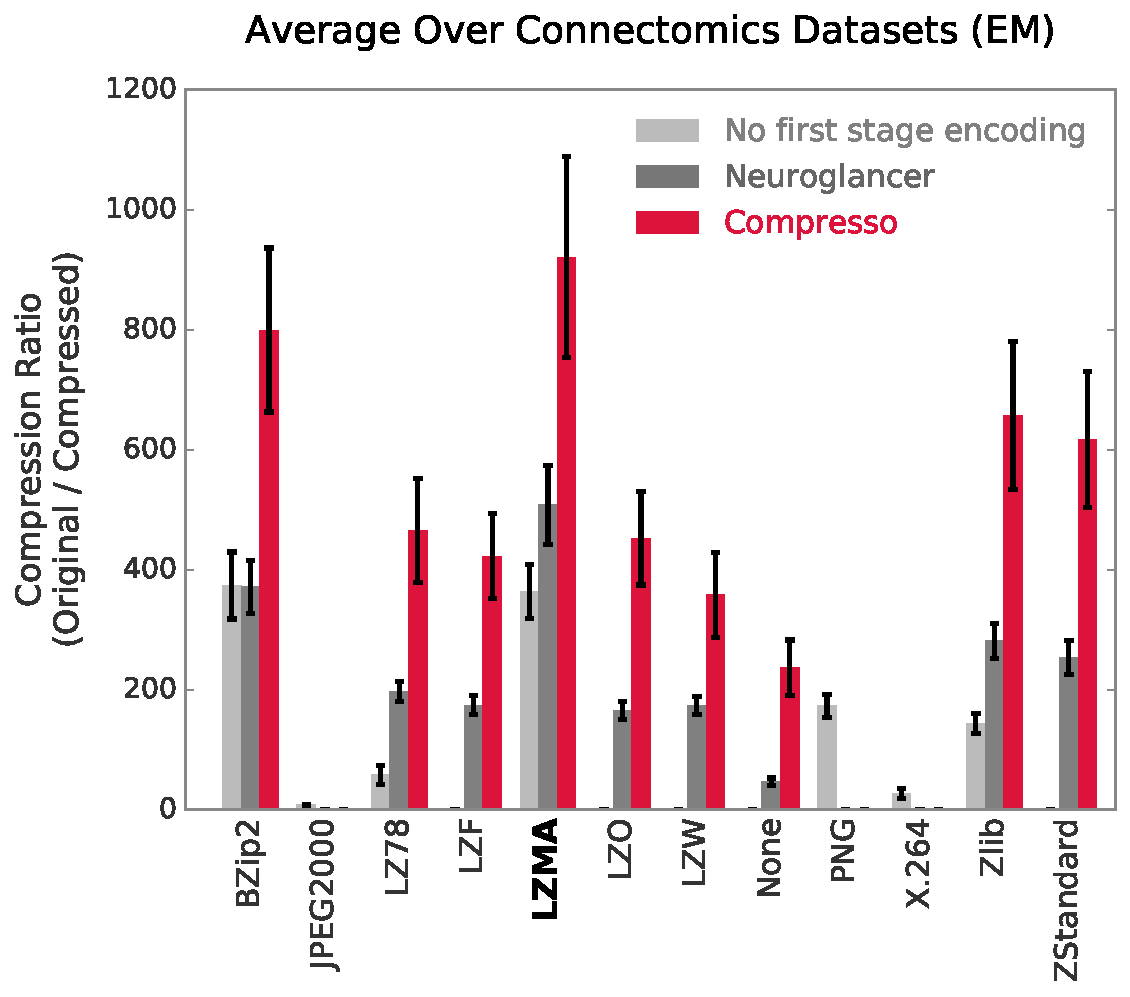
\includegraphics[width=0.5\textwidth]{gfx/LCylinder+ac3+ac4+cremiA+cremiB+cremiC_rhoana_compression_ratios.pdf}%
		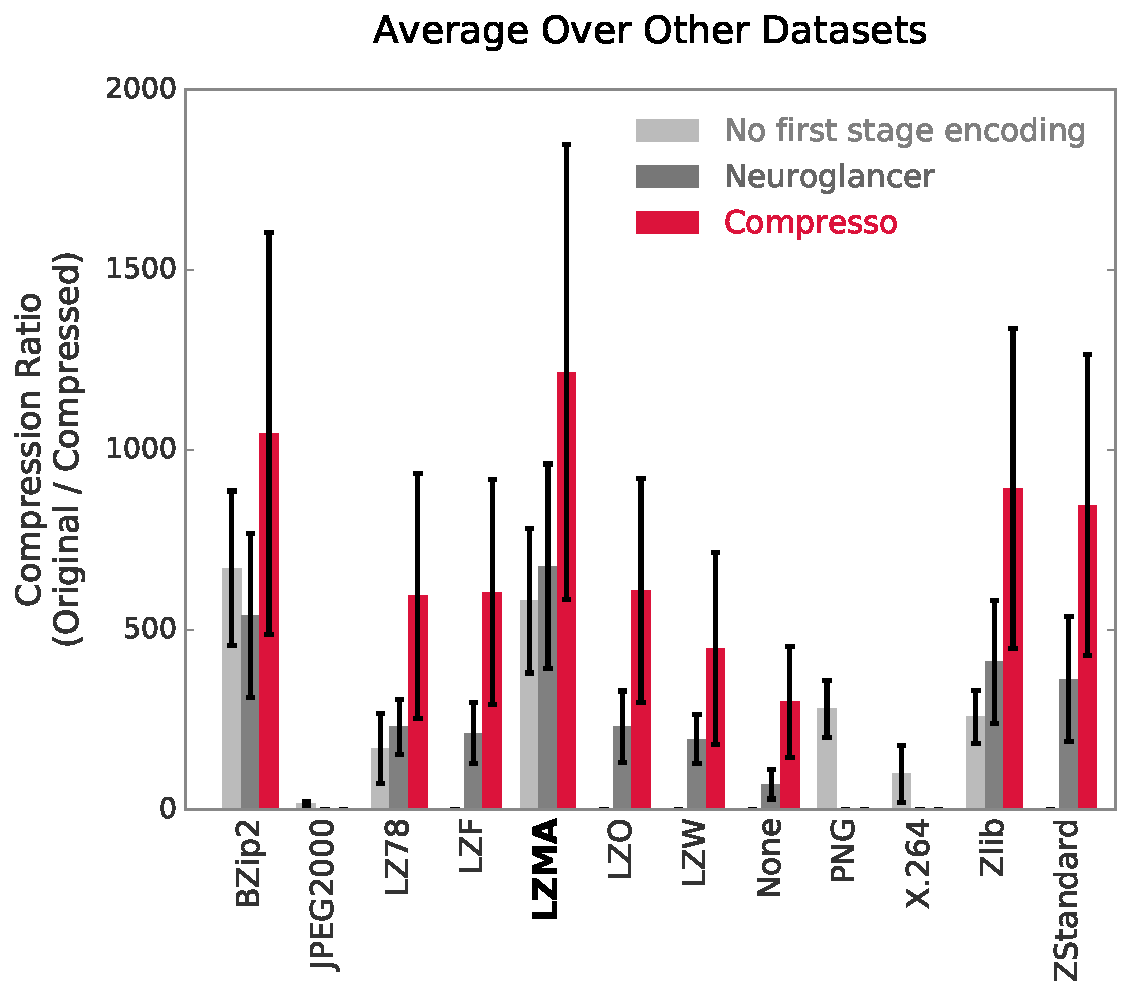
\includegraphics[width=0.5\textwidth]{gfx/VOC+mri1+mri2+mri3+BSD_gold_compression_ratios.pdf}%
		\caption{Compression ratios of general-purpose compression methods combined with \appName and Neuroglancer. % on all connectomics datasets (left) and on the other datasets (right).
%		the average on the remaining five connectomics datasets (right).
		\appName paired with LZMA yields the best compression ratios for all connectomics datasets and in average (four out of five) for the others.}
		\label{fig:compression_ratios}
	\end{center}
	\vspace{-18pt}
\end{figure}




%\vspace{-0.2cm}

\noindent of our requirement of lossless compression. It performs better when information loss is tolerated, however, even then it does not surpass the more specialized encoding schemes. These observations also hold for JPEG2000 and PNG. \appName with LZMA outperforms all other existing methods on connectomics datasets by 80\%. 

The fundamental principles guiding \appName are valid for a diverse set of segmentation datasets (Fig.~\ref{fig:compression_ratios}, right). We evaluate the performance of our compression scheme on three MRI and two image segmentation datasets to demonstrate additional potential use cases. \appName followed by LZMA compresses the MRI datasets reasonably well, particularly on the SPL Knee Atlas which contains highly redundant boundary segments.
%\appName followed by LZMA compresses the SPL Brain Atlas data by nearly a factor of 640x. 
The Berkeley Segmentation and PASCAL Visual Object Class datasets are two very common benchmarks in image segmentation~\cite{MartinFTM01,pascal-voc-2012}. Currently these datasets use GZIP and PNG compression but \appName with LZMA can improve on them by a factor of over 10x and 5x respectively. 

In terms of speed, \appName is on par with Neuroglancer across all datasets and achieves throughput of 112.16 megabytes per second ($SD = 18.62$ MB/s) for compression and 222.85 megabytes per second ($SD = 32.14$ MB/s) for decompression. All experiments ran on a single core of a Intel Xeon 2.3GHz CPU.

%Compared to all other methods, X.264 performs surprisingly poor on these datasets. Our requirement of lossless compression prevents this method from eliminating high frequencies between successive frames. We found that the video compression performs much better when information loss is tolerated. However, even then, the technique does not surpass the specialized encoding schemes discussed. These observations are also valid for JPEG2000 and PNG because of similar data assumptions.
 %The decompression speed for \appName was worse than the other encoding algorithms. However, there is significant room for optimization.
